

\documentclass{article}
\usepackage{graphicx}
\begin{document}
\section*{NumPy array manipulation}
A grayscale image can be thought of as a rectangular matrix, with each element
representing the intensity at the corresponding pixel. \newline
\begin{figure}[h]
\begin{center}
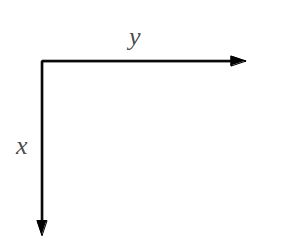
\includegraphics[height=100pt]{../pictures/image_axes.png}
\caption{Co-ordinate axes for images loaded from matrices}
\end{center}
\end{figure}
\newline
Load \texttt{pup.txt} into Python as a NumPy array using the \texttt{numpy.loadtxt} 
function; this is a rectangular matrix that describes the below image:
\newline
\begin{figure}[h]
\begin{center}
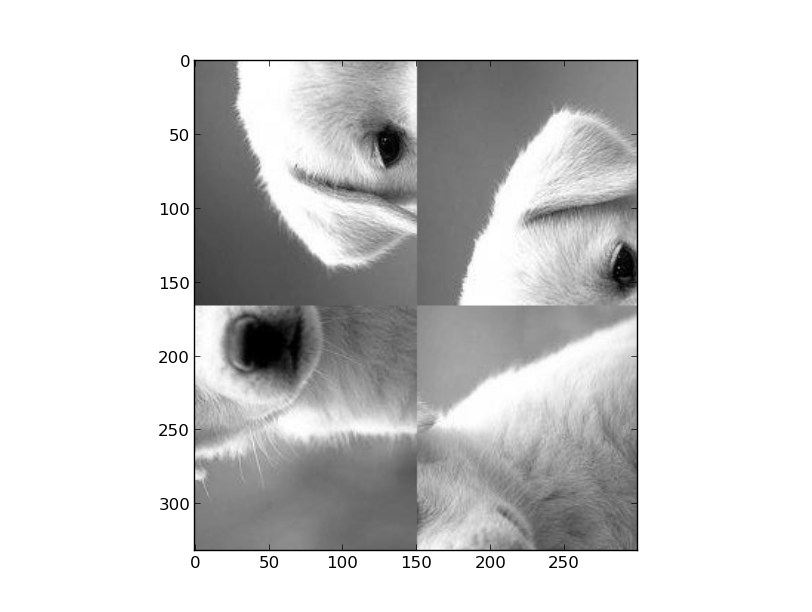
\includegraphics[height=200pt, width=275pt]{pup.png}
\caption{Your worst nightmare}
\end{center}
\end{figure}

Write a program that rearranges the pieces of this image. Looking at \texttt{
pup.txt}, you will note that 0 and 1 represent `black' and `white' respectively,
with all values in between corresponding to increasingly lighter shades of gray.
\end{document}
